%% ============================================================
%% CBCTQ 2026 - Extended Abstract (Poster Session)
%% Two-Column Format (Up to 2 pages)
%% ============================================================

\documentclass{cbctq}

\usepackage[english]{babel}
\usepackage[utf8]{inputenc}
\usepackage{amsmath,amssymb,amsfonts}
\usepackage{graphicx}
\usepackage{cite}
\usepackage{braket}

% figuras geradas pelo plots.py; figs/ local (Overleaf) ou ../figs/ (repo)
\graphicspath{{figs/}{../figs/}{./}}

% ------------------------------------------------------------
% Header
% ------------------------------------------------------------
\usepackage{fancyhdr}
\pagestyle{fancy}
\fancyhf{}
\setlength{\headheight}{28pt}

\fancyhead[L]{\raisebox{-0.2\height}{
\includegraphics[height=22pt]{cbctq2026-logo.png}}}

\fancyhead[C]{\footnotesize
Congresso Brasileiro de Ciências e Tecnologias Quânticas (CBCTQ 2026) --
September 21--25, 2026, Innovation District of Cantareira, Niterói--RJ, Brazil}

\fancyhead[R]{\footnotesize\thepage}

\renewcommand{\headrulewidth}{0.4pt}
\renewcommand{\footrulewidth}{0pt}

% First page style
\fancypagestyle{plain}{
  \fancyhf{}
  \setlength{\headheight}{28pt}
  \fancyhead[L]{\raisebox{-0.2\height}{
\includegraphics[height=22pt]{cbctq2026-logo.png}}}
  \fancyhead[C]{\footnotesize
  Congresso Brasileiro de Ciências e Tecnologias Quânticas (CBCTQ 2026) --
  September 21--25, 2026, Innovation District of Cantareira, Niterói--RJ, Brazil}
  \fancyhead[R]{\footnotesize\thepage}
  \renewcommand{\headrulewidth}{0.4pt}
}

% Força os títulos para inglês
\makeatletter
\renewcommand{\@WORDappendix}{Appendix}
\renewcommand{\@WORDreferences}{References}
\renewcommand{\@WORDproof}{Proof}
\makeatother

% ------------------------------------------------------------
\begin{document}

\title{Are quantum-inspired evolutionary algorithms competitive for QAOA
parameter optimization? A Max-Cut benchmark}

\author{
Victor Brasil, João Vitor, and Leandro C. Souza%
\thanks{
The authors are with the Centro de Informática, Universidade Federal da
Paraíba (UFPB), João Pessoa, PB, Brazil.
E-mail: \texttt{victor.henrique72@gmail.com}.
}
}

\maketitle

\markboth{Congresso Brasileiro de Ciências e Tecnologias Quânticas (CBCTQ 2026) -- September 21--25, 2026, Innovation District of Cantareira, Niterói--RJ, Brazil}{}

% ============================================================
\begin{abstract}
% [PLACEHOLDER — uma linha; prosa do Victor]
We benchmark a quantum-inspired evolutionary algorithm against classical optimizers for QAOA parameter optimization on Max-Cut.
\end{abstract}

\begin{keywords}
% [PLACEHOLDER — uma linha; prosa do Victor]
QAOA, quantum-inspired evolutionary algorithm, Max-Cut, parameter optimization, NISQ.
\end{keywords}

% ============================================================
\section{Introduction}
% [PLACEHOLDER — contexto, motivação, objetivo e pergunta de pesquisa.
%  Citar QAOA \cite{farhi2014qaoa}, NISQ \cite{preskill2018nisq},
%  QIEA \cite{han2002qiea}. Prosa do Victor.]
[Introduction placeholder.]

% ============================================================
\section{Methodology}
% [PLACEHOLDER — QAOA Max-Cut, QIEA com codificação em bits, baselines,
%  protocolo de orçamento justo. Uma ou duas equações no máximo. Prosa do Victor.]
[Methodology placeholder.]

\begin{equation}
H_C = \sum_{(i,j)\in E} \tfrac{1}{2}\,(1 - Z_i Z_j).
\end{equation}

% ============================================================
\section{Preliminary Results}
% [PLACEHOLDER — leitura da figura de convergência e p-valor do Wilcoxon.
%  Prosa do Victor.]
[Preliminary results placeholder.]

\begin{figure}[t]
\centering
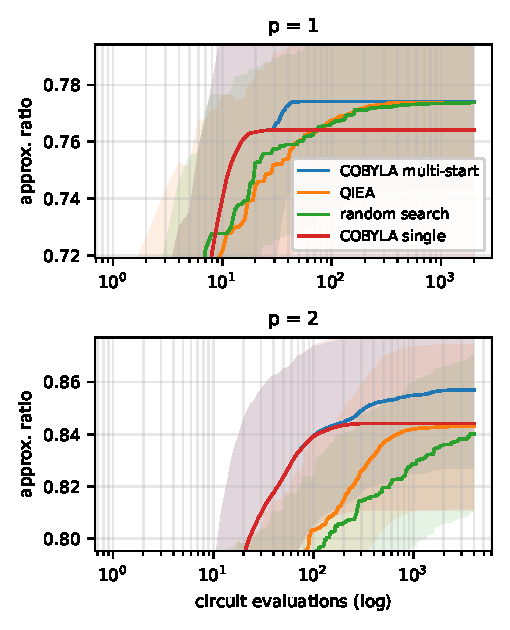
\includegraphics[width=\linewidth]{convergence.pdf}
\caption{% [PLACEHOLDER caption — prosa do Victor]
Mean approximation ratio versus circuit evaluations (deviation band) for
$p=1$ and $p=2$, comparing QIEA, COBYLA single-start, COBYLA multi-start,
and random search under an equal evaluation budget.}
\label{fig:convergence}
\end{figure}

% --- Figura opcional de estabilidade: ativar se couber em 2 páginas ---
% \begin{figure}[t]
% \centering
% 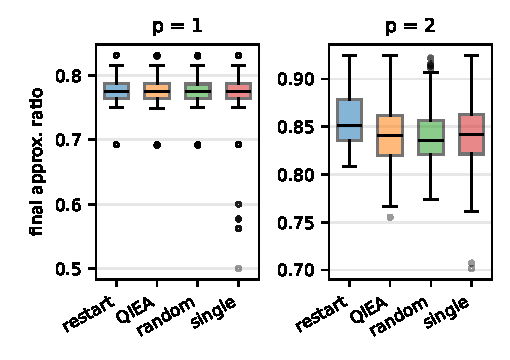
\includegraphics[width=\linewidth]{stability.pdf}
% \caption{[PLACEHOLDER] Distribution of final approximation ratio per
% optimizer, showing the failure tail of single-start COBYLA.}
% \label{fig:stability}
% \end{figure}

% ============================================================
\section{Discussion and Future Work}
% [PLACEHOLDER — observações, limitação de escala/simulação clássica,
%  ponte pro QGA gate-based na era NISQ. Prosa do Victor.]
[Discussion placeholder.]

% ============================================================
\nocite{*}
\bibliographystyle{IEEEtran}
\bibliography{refs}

\end{document}
